\chapter{Contracción por Bisimulación}

Como hemos mencionado a lo largo de este trabajo, la noción de bisimulación nos permite relacionar modelos lógicamente equivalentes a partir de 
características estructurales entre sí. En el capítulo anterior, determinamos qué tan complejo es decidir si existe una bisimulación entre dos 
modelos.

Otra pregunta que surge a la hora de estudiar una lógica modal y su respectiva noción de bisimulación es:
Dado un modelo, ¿Existe un procedimiento capaz de encontrar otro modelo que sea bisimilar?. Más aún, ¿Podría dicho procedimiento encontrar 
un modelo de tamaño mínimo entre todos los modelos bisimilares al modelo original?.

En la lógica modal básica la respuesta a esta pregunta es positiva, y al modelo encontrado se lo llama la contracción por bisimulación.
Como se presenta en \cite[Capítulo 3]{HandbookModalLogic}, la contracción se define a partir del estudio de las autobisimulaciones del modelo. En particular,
se demuestra que la unión de dos bisimulaciones es también una bisimulación, de allí se obtiene que existe una autobisimulación máxima de un modelo.

Luego, se demuestra que dicha autobisimulación máxima es una relación de equivalencia, por lo que se puede definir un modelo cuyo dominio sea el cociente
del dominio del modelo original con respecto a su autobisimulación máxima, donde cada punto representa una clase de equivalencia de dicha autobisimulación, y donde 
dos clases de equivalencia se relacionan entre sí cuando existen dos puntos de dichas clases que se relacionaban en el modelo original.

Finalmente se concluye que dicha contracción satisface que cada punto del modelo original es bisimilar al punto que representa su clase de equivalencia, y 
que, a su vez, es de tamaño mínimo entre todos los modelos bisimilares.

Habiendo mencionado un poco la ruta de trabajo seguida para la lógica modal básica, intentaremos realizar un estudio similar para la lógica de `Knowing-How' basada en 
incertidumbre.

\section{Primera Propuesta de Contracción}

\begin{definicion}
    Sea $\model=\tup{\W,\R,\cset{\S_i}_{i \in \AGT},\V,\ACT}$ un \ults, y $Z \subseteq \W \times \W$ entonces decimos que
    \begin{center}
        $Z$ es una autobisimulación de $\modults$ si y sólo si $Z$ es una \KHilogic-bisimulación        
    \end{center}
\end{definicion}

Recordemos la definición de $A_\modults$ y de $\rho_\modults$, introducida en \ref{def:Am}, y veamos el siguiente teorema 
que caracteriza la autobisimulación máxima de un \ults.

\begin{teorema}
    Sea $\model=\tup{\W,\R,\cset{\S_i}_{i \in \AGT},\V,\ACT}$ un \ults, entonces se cumple que:
    \begin{itemize}
        \item $A_\modults$ es una autobisimulación de $\modults$.
        \item Sea $Z \subseteq \W \times \W$ una autobisimulación de $\modults$ entonces $Z \subseteq A_\modults$. 
        Es decir, $A_\modults $ es la autobisimulación máxima de $\modults$. 
    \end{itemize}
\end{teorema}

\begin{demostracion}
    Sea $\model=\tup{\W,\R,\cset{\S_i}_{i \in \AGT},\V,\ACT}$ un \ults, probaremos ambas propiedades por separado:

    \begin{itemize}
        \item Queremos ver que $A_\modults$ es una autobisimulación de $\modults$, para ello debemos verificar que:
        \begin{itemize}
            \item (Atom) Dado $(w,v) \in A_\modults$, por definición de $A_\modults$, se cumple que $\V(w) = \V(v)$.
            \item (A-Zig) Notemos que $A_\modults$ es una relación de equivalencia, luego para cada $w\in \W$ se cumple que $(w,w) \in A_\modults$.
            \item (A-zag) Podemos utilizar el mismo argumento que en (A-zig) para demostrar este caso.
            \item ($\khi$-zig) Sea $U \subseteq \W$ tal que para cada $s \in \rho_\modults$ se cumple que $s \cap U = \emptyset$ o 
            $s \subseteq U$, si $U \ultsExecAgi T$ para algún $T \subseteq \W$, entonces existe $T' \subseteq \W$ tal que
                \begin{multicols}{2}
                    \begin{itemize}
                        \item $A_\modults(U) \ultsExecAgi T'$, 
                        \item $T' \subseteq A_\modults(T)$.
                    \end{itemize}
                \end{multicols}

            Sean $U,T$ subconjuntos de $\W$ tales que $U \ultsExecAgi T$ y $U$ es tal que para cada $s \in \rho_\modults$ se cumple que 
            $s \cap U = \emptyset$ o $s \subseteq U$, queremos encontrar $T' \subseteq \W$ que cumpla lo mencionado.
            
            Demostremos por un lado que $U = A_\modults(U)$:
            
            ($\subseteq$) Siguiendo el argumento usado en (A-Zig), es claro que para $w \in U$ se cumple que $w \in A_\modults(U)$, 
            pues $(w,w) \in A_\modults$ para cada $w \in \W$. 
            
            ($\supseteq$) Sea $v \in A_\modults(U)$, queremos ver que $v \in U$.
            Como $v \in A_\modults(U)$, entonces existe $w \in U$ tal que $(w,v) \in A_\modults$ y, por lo tanto, $v \in [w]$.
            
            Como $w \in U$ entonces $[w] \subseteq U$. Luego $v \in U$.

            Entonces demostramos que $U = A_\modults(U)$.

            Notemos que siendo $X \subseteq \W$ entonces $X \subseteq A_\modults(X)$, pues como analizamos anteriormente 
            $(w,w) \in A_\modults$ para cada $w \in \W$.

            Juntando lo mencionado, podemos afirmar que $T' = T$ cumple que:

             \begin{itemize}
                \item $A_\modults(U) \ultsExecAgi T'$, pues dijimos $A_\modults(U) = U$, y por hipótesis, $U \ultsExecAgi T = T'$.  
                \item $T' \subseteq A_\modults(T')$ pues esto se cumple para todo $X \subseteq \W$.
            \end{itemize}
            Luego queda demostrado que $A_\modults$ satisface ($\khi$-zig).

            \item ($\khi$-zag) Análogo a ($\khi$-zig), pues notemos que como $A_\modults$ es una relación de equivalencia, es simétrica.
        \end{itemize}

        Luego $A_\modults$ es una autobisimulación de $\modults$.
        
        \item Queremos ver que dada $Z \subseteq \W \times \W$ autobisimulación de $\modults$, entonces $Z \subseteq A_\modults$.
        
        Supongamos que no es cierto, es decir, existe $Z \subseteq \W \times \W$ autobisimulación de $\modults$ tal que hay 
        $w,v \in \W$ que cumplen que $(w,v) \in Z$ y $(w,v) \notin A_\modults$. 

        Como $Z$ es una autobisimulación entonces satisface (Atom), es decir, $\V(w) = \V(v)$. Pero notemos que por definición de 
        $A_\modults$, $(w,v) \in A_\modults$, lo cuál es absurdo, pues dijimos que $(w,v) \notin A_\modults$.

        El absurdo vino de suponer que $Z \nsubseteq A_\modults$.    
    \end{itemize}
    Luego queda demostrada la propiedad.
\end{demostracion}

Una primera observación que surge a partir de este teorema es que, a diferencia de lo mencionado sobre el caso de la lógica modal básica, 
encontramos una forma de identificar la autobisimulación máxima de un modelo sin necesidad de demostrar que la unión preserva bisimulación. 

En particular, se demuestra que la partición de nodos de acuerdo a la función de valuación $\V$ siempre es una autobisimulación.

Entonces sea $\modults$ un \ults, nos gustaría definir su contracción por bisimulación a partir de $A_\modults$, su autobisimulación máxima.

Tomando un camino similar al de la lógica modal básica, una posible propuesta sería un modelo en el que se tenga como dominio al cociente 
del dominio de $\modults$ con respecto a $A_\modults$ y se relacione a las clases de equivalencia $[w], [v] \in \rho_\modults$ siempre que 
$w, v$ estén relacionados en $\modults$. Por otro lado, la relación de indistinguibilidad de cada agente y el conjunto de acciones de $\modults$ se conservarían.

Sin embargo consideremos el siguiente modelo (\Cref{fig:1stproposaloriginal}):

% \begin{figure}[h]
%     \centering
%     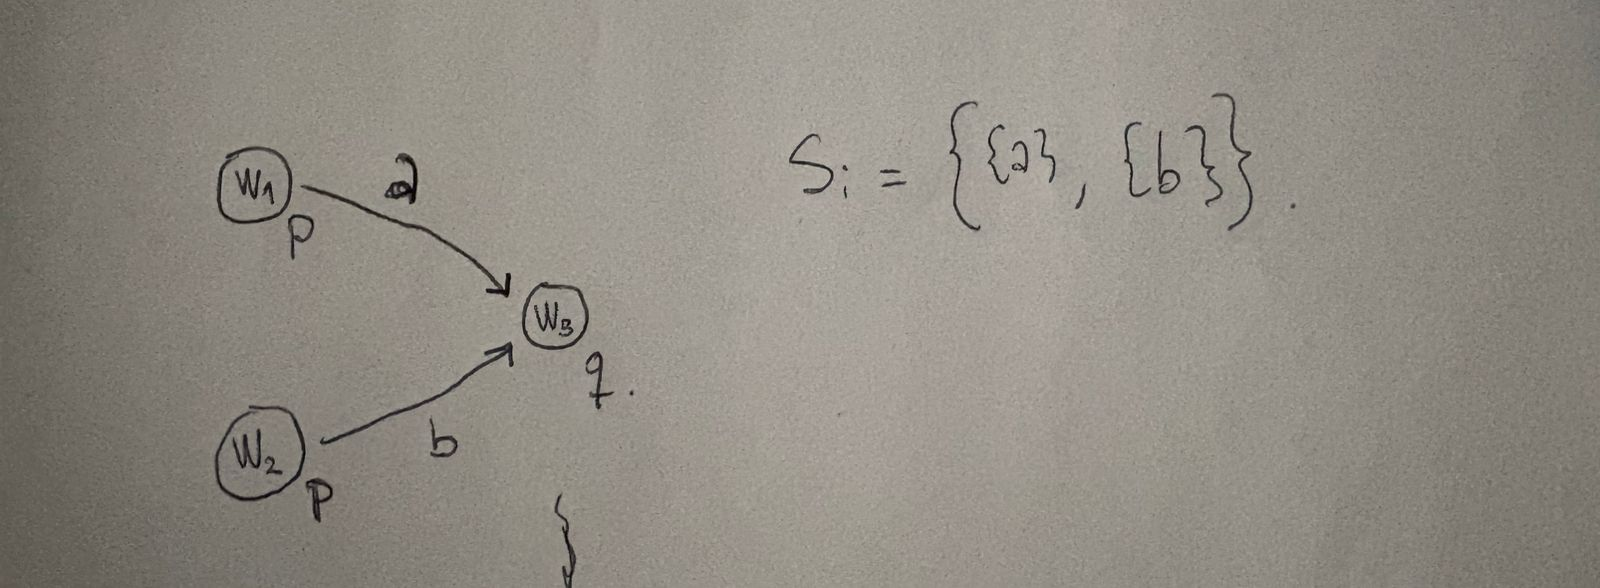
\includegraphics[width=0.5\textwidth]{imagenes/1ra_propuesta_original.jpeg}
%     \caption{$\modults$}
%     \label{fig:1stproposaloriginal}
% \end{figure}

\begin{figure}[h]
    \hspace{3.4cm}
    \vspace{0.1cm}
    \begin{tikzpicture}
        \node[state] (p) {$p$};
        \node[state, below of=p, yshift=-1.5cm] (p2) {$p$};
        \node[state, right of=p, yshift=-1cm, xshift=1.5cm] (q) {$q$};
        
        \node at ($(p)+(0,0.5)$) {$w_1$};
        \node at ($(q)+(0,0.5)$) {$w_3$};
        \node at ($(p2)+(0.05,-0.6)$) {$w_2$};

        \path (p) edge [bend left] node [above] {$a$} (q);
        \path (p2) edge [bend right] node [above] {$b$} (q);
    \end{tikzpicture}
    \hspace{1cm}
    \raisebox{1.8cm}{
        \begin{minipage}{0.45\textwidth}
            $\S_i = \left\{
                \begin{array}{c}
                    \{a\}, \{b\}
                \end{array}
            \right\}$
        \end{minipage}
    }
    \caption{Representación gráfica de $\modults$}
    \label{fig:1stproposaloriginal}
\end{figure}

Con esta propuesta de contracción ($\modults'$), obtendríamos el modelo (\Cref{fig:1stproposalcontraction}):

% \begin{figure}[h]
%     \centering
%     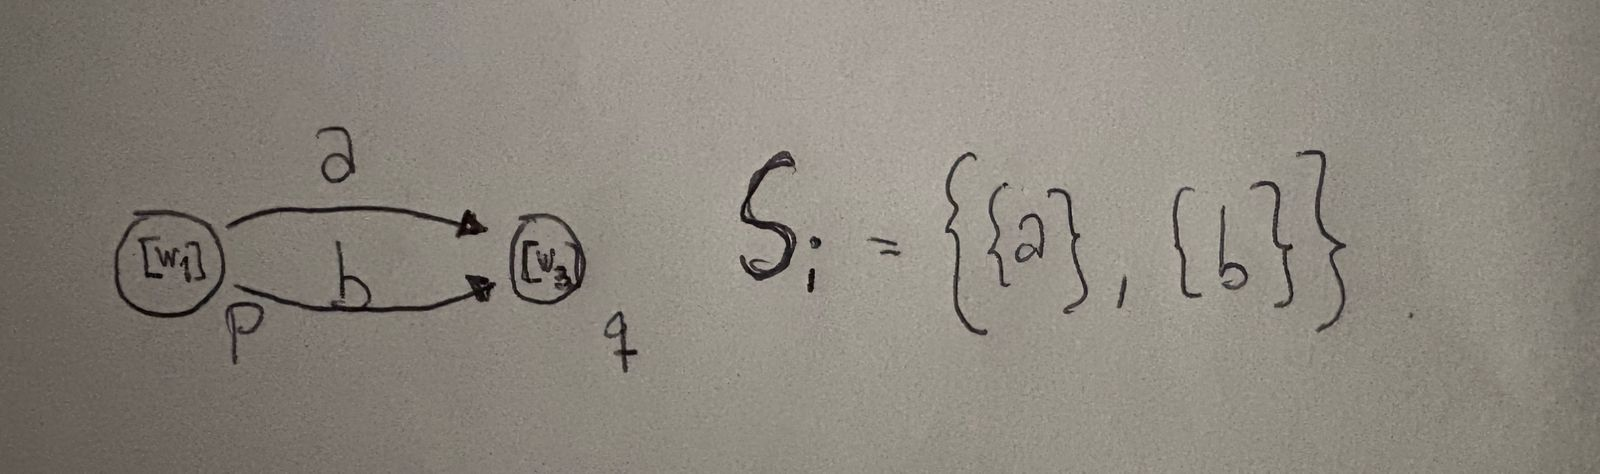
\includegraphics[width=0.5\textwidth]{imagenes/1ra_propuesta_contraido.jpeg}
%     \caption{$\modults'$}
%     \label{fig:1stproposalcontraction}
% \end{figure}

\begin{figure}[h]
    \hspace{3.2cm}
    \vspace{0.8cm}
    \begin{tikzpicture}
        \node[state] (p) {$p$};
        \node[state, right of=p, xshift=1.5cm] (q) {$q$};
        
        \node at ($(p)+(0,0.6)$) {$[w_1]$};
        \node at ($(q)+(0,0.6)$) {$[w_3]$};

        \path (p) edge [bend left] node [above] {$a$} (q)
              (p) edge [bend right] node [above] {$b$} (q);
    \end{tikzpicture}
    \hspace{1cm}
    \raisebox{0.4cm}{
        \begin{minipage}{0.45\textwidth}
            $\S'_i = \left\{
                \begin{array}{c}
                    \{a\}, \{b\}
                \end{array}
            \right\}$
        \end{minipage}
    }
    \caption{Representación gráfica de $\modults'$}
    \label{fig:1stproposalcontraction}
\end{figure}

Notemos que $\modults, w_1 \not\models \khi(p,q)$ pero $\modults', [w_1] \models \khi(p,q)$, luego $\modults,w_1$ y 
$\modults',[w_1]$ no son bisimilares.

Por lo que esta contracción por bisimulación no sería adecuada, ya que no produce un modelo bisimilar al modelo original.

Otra posible propuesta sería restringir más la relación entre las puntos del modelo contraído. Es decir, relacionar las clases 
$[w], [v] \in \rho_\modults$ cuando para cada $w' \in [w]$ existe $v' \in [v]$ tal que $w'$ y $v'$ están relacionados en el modelo original.

Luego consideremos el siguiente modelo (\Cref{fig:2ndproposaloriginal}):

% \begin{figure}[h]
%     \centering
%     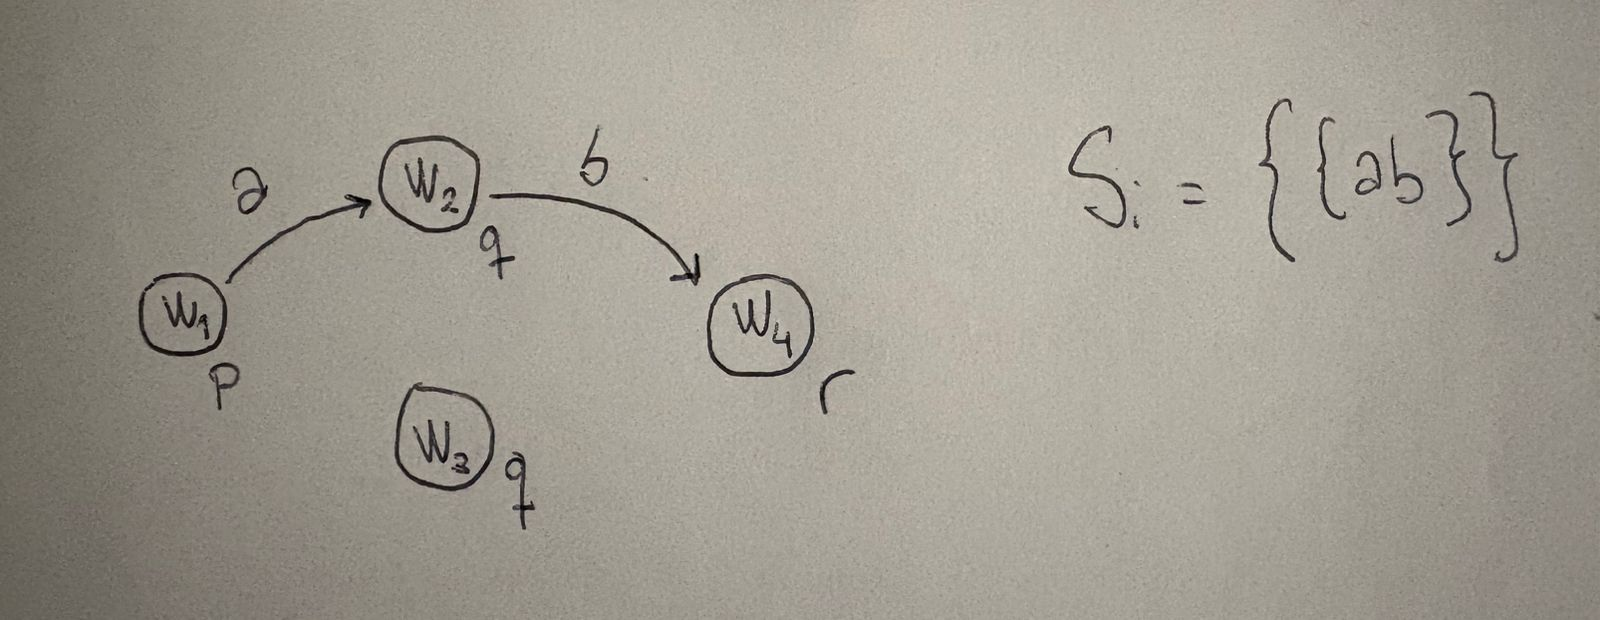
\includegraphics[width=0.5\textwidth]{imagenes/2da_propuesta_original.jpeg}
%     \caption{$\modults$}
%     \label{fig:2ndproposaloriginal}
% \end{figure}

\begin{figure}[h]
    \hspace{2.6cm}
    \vspace{0.2cm}
    \begin{tikzpicture}
        \node[state] (p) {$p$};
        \node[state, right of=p, yshift=1cm, xshift=1.5cm] (q) {$q$};
        \node[state, below of=q, yshift=-1.5cm] (q2) {$q$};
        \node[state, right of=p, xshift=3.5cm] (r) {$r$};
        
        \node at ($(p)+(0,0.5)$) {$w_1$};
        \node at ($(r)+(0,0.5)$) {$w_4$};
        \node at ($(q)+(0,0.5)$) {$w_2$};
        \node at ($(q2)+(0.05,-0.6)$) {$w_3$};

        \path (p) edge [bend left] node [above] {$a$} (q);
        \path (q) edge [bend left] node [above] {$b$} (r);
    \end{tikzpicture}
    \hspace{1cm}
    \raisebox{1.8cm}{
        \begin{minipage}{0.45\textwidth}
            $\S_i = \left\{
                \begin{array}{c}
                    \{ab\}
                \end{array}
            \right\}$
        \end{minipage}
    }
    \caption{Representación gráfica de $\modults$}
    \label{fig:2ndproposaloriginal}
\end{figure}


Y su contracción por bisimulación con la propuesta mencionada (\Cref{fig:2ndproposalcontraction}):

% \begin{figure}[h]
%     \centering
%     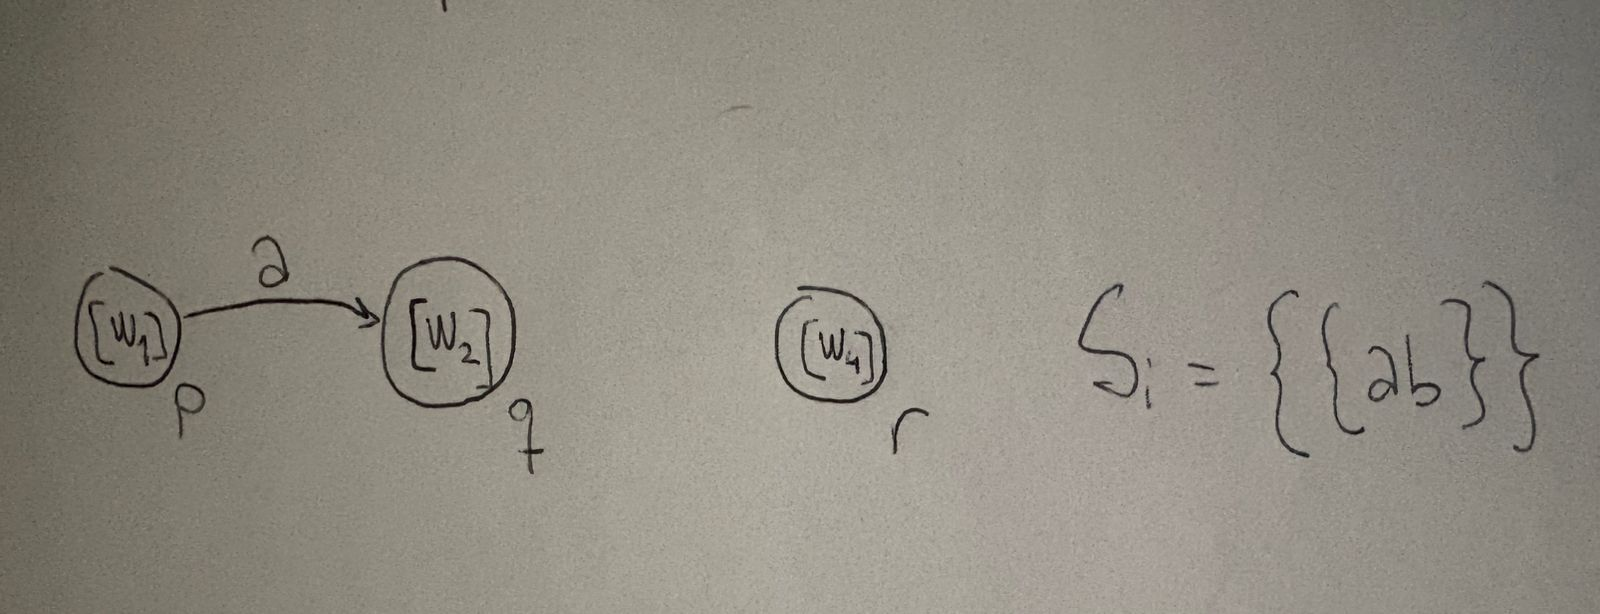
\includegraphics[width=0.5\textwidth]{imagenes/2da_propuesta_contraido.jpeg}
%     \caption{$\modults'$}
%     \label{fig:2ndproposalcontraction}
% \end{figure}



\begin{figure}[h]
    \hspace{2.54cm}
    \vspace{0.4cm}
    \begin{tikzpicture}
        \node[state, yshift=-1cm] (p) {$p$};
        \node[state, right of=p, xshift=1.5cm] (q) {$q$};
        \node[state, right of=p, xshift=3.5cm] (r) {$r$};
        
        \node at ($(p)+(0,0.75)$) {$[w_1]$};
        \node at ($(r)+(0,0.75)$) {$[w_4]$};
        \node at ($(q)+(0,0.75)$) {$[w_2]$};

        \path (p) edge [bend left] node [above] {$a$} (q);
    \end{tikzpicture}
    \hspace{0.82cm}
    \raisebox{0.14cm}{
        \begin{minipage}{0.45\textwidth}
            $\S'_i = \left\{
                \begin{array}{c}
                    \{ab\}
                \end{array}
            \right\}$
        \end{minipage}
    }
    \caption{Representación gráfica de $\modults'$}
    \label{fig:2ndproposalcontraction}
\end{figure}

Si analizamos ambos modelos, podemos notar que $\modults,w_1 \models \khi(p,r)$ pero $\modults',[w_1] \not\models \khi(p,r)$, luego 
$\modults,w_1$ y $\modults',[w_1]$ no son bisimilares.

Por lo que esta propuesta tampoco es adecuada, ya que tampoco produce un modelo bisimilar al modelo original.

Si analizamos ambos contraejemplos, podemos notar que la primera propuesta de contracción podría agregar caminos fuertemente ejecutables al modelo 
y la segunda podría eliminar caminos fuertemente ejecutables del modelo. Los fallos de ambas propuestas nos dan la idea de que no parece 
existir una contracción directa en la cuál no se modifique la relación de indistinguibilidad de cada agente y las acciones 
consideradas por el modelo. 

A partir de lo mencionado, surge la siguiente propuesta de contracción, la cuál modifica el conjunto de acciones y la relación de indistinguibilidad 
de cada agente.


\begin{definicion}
    Sea $\model=\tup{\W,\R,\cset{\S_i}_{i \in \AGT},\V,\ACT}$ un \ults. Se define su contracción por bisimulación, $\model'=\tup{\W',\R',\cset{\S_i'}_{i \in \AGT'},\V',\ACT'}$ donde 
    \begin{center}
        \begin{itemize}
            \item $\W' := \W/A_\modults$
            \item $\R' := \{\R'_{a_\sigma} \subseteq \W' \times \W' \mid a_\sigma \in \ACT'\}$ donde $([w],[v]) \in \R'_{a_\sigma}$ si y sólo si
            \begin{enumerate}
                \item existen $w' \in [w]$ y $v' \in [v]$ tal que $(w',v')\in \R_\sigma$
                \item $\sigma$ es fuertemente ejecutable para cada $w' \in [w]$.
            \end{enumerate}
            \item $\S_i' := \{ \pi' = \{a_\sigma \mid \sigma \in \pi\} \mid \pi \in \S_i \}$
            \item $\V'([w]) := \V(w)$
            \item $\ACT' := \{a_\sigma \mid $ existe $ \pi\in \S_i$ tal que $ \sigma \in \pi$ para algún $i \in \AGT \}$ 
        \end{itemize}
    \end{center}
\end{definicion}
    
Una vez presentada la contracción, nos gustaría asegurarnos que, efectivamente, construye un modelo bisimilar. Para ello demostraremos el 
siguiente teorema.

\begin{teorema}
    Sea $\model=\tup{\W,\R,\cset{\S_i}_{i \in \AGT},\V,\ACT}$ un \ults y sea $\modults'$ su contracción por bisimulación entonces 
    $\tup{\modults,w}$ y $\tup{\modults',[w]}$ son $\KHilogic$-bisimilares para cada $w \in \W$.
\end{teorema}

\begin{demostracion}
    Sea $\model=\tup{\W,\R,\cset{\S_i}_{i \in \AGT},\V,\ACT}$ un \ults
    y sea $\modults'$ su contracción por bisimulación, basta ver que $Z = \{(w,[w]) \in \W \times\W'\}$ es una \KHilogic-bisimulación para demostrar la propiedad.

    Dado que $\W$ es no vacío entonces es claro que $Z$ es no vacío también.

    Por otro lado, notemos que por la definición de $\V'$, es claro que $Z$ satisface (Atom).

    A su vez, por cómo definimos $Z$, es fácil ver que también (A-zig) y (A-zag) son satisfechos.
    
    Demostremos entonces que se satisfacen ($\khi$-zig) y ($\khi$-zag).

    \begin{itemize}
        \item ($\khi$-zig) Sean $U, T$ subconjuntos de $\W$ tales que $U \ultsExecAgi T$ y para cada $s \in \rho_\modults$ se cumple que 
        $s \subseteq U$ o $s \cap U = \emptyset$, queremos encontrar $T' \subseteq \W'$ que

        \begin{multicols}{2}
            \begin{itemize}
                \item $Z(U) \ultsExecAgi T'$, 
                \item $T' \subseteq Z(T)$.
            \end{itemize}
        \end{multicols}

        Veamos que $T' := \{ [w] \mid w \in T\}$ cumple con lo mencionado. Por como definimos $Z$, es claro que $T'  = Z(T)$, por lo que 
        $T' \subseteq Z(T)$. Entonces demostremos $Z(U) \ultsExecAgi T'$.

        Como $U \ultsExecAgi T$, existe $\pi \in S_i$ tal que cada plan de $\pi$ es fuertemente ejecutable en cada nodo de $U$ y 
        $\R_\pi(U) \subseteq T$. 

        Sabemos por la definición de $\modults'$ que existe $\pi' = \{a_\sigma \mid \sigma \in \pi\} \in S_i'$. Demostraremos que $\pi'$ 
        atestigua $Z(U) \ultsExecAgi T'$, es decir, que cada $a_\sigma \in \pi$ es fuertemente ejecutable en $Z(U)$ y que además 
        $\R'_{\pi'}(Z(U)) \subseteq T'$.

        Sea $[w] \in Z(U)$, veamos que $\pi'$ es fuertemente ejecutable en $[w]$. Sea $a_\sigma \in \pi'$, queremos ver que $a_\sigma$ es fuertemente 
        ejecutable en $[w]$. Notar que cómo $a_\sigma$ es un plan de un solo paso, solo basta con ver que exista $[v] \in \W'$  tal que 
        $([w],[v]) \in \R'_{a_\sigma}$.
        
        Primero notemos que como $[w] \in Z(U)$, entonces existe $w' \in [w]$ tal que $w' \in U$. Luego, por la hipótesis sobre $U$
        se cumple que $[w'] = [w] \subseteq U$. Pero veamos que como $\pi$ es fuertemente ejecutable en $U$ entonces es fuertemente ejecutable en cada nodo 
        de $[w]$, por lo que existe $v' \in \W$ tal que $v \in \R_\sigma(w')$. Como $\sigma$ es fuertemente en todo $[w]$ y $(w',v') \in \R_\sigma$, entonces 
        $([w],[v']) \in \R'_{a_\sigma}$. Queda demostrado entonces que $\pi'$ es fuertemente ejecutable en $Z(U)$.
        
        Demostraremos ahora que $\R'_{\pi'}(Z(U)) \subseteq T'$.

        Sea $[v] \in \R'_{\pi'}(Z(U))$, entonces existe $[w] \in Z(U)$ y $a_\sigma \in \pi'$ tal que $([w],[v]) \in \R'_{a_\sigma}$. Notar que 
        como $[w] \in Z(U)$, entonces existe $w' \in [w]$ tal que $w' \in U$ y, por lo tanto, $[w'] = [w] \subseteq U$. Si analizamos la definición 
        de $\R'_{a_\sigma}$, como $([w],[v]) \in \R'_{a_\sigma}$ entonces existen $w'' \in [w]$ y $v'' \in [v]$ tal que $(w'',v'') \in \R_\sigma$.
        Como $w'' \in U$ y $\R_\pi(U) \subseteq T$, entonces se cumple que $v'' \in T$, lo que nos dice que $[v''] = [v] \in T'$, que era lo que 
        queríamos demostrar. Luego $\R'_{\pi'}(Z(U)) \subseteq T'$. 

        Queda demostrado entonces que $Z$ satisface $\khi$-zig.

        \item ($\khi$-zag) Sean $U', T' \in \W'$ tales que $U' \ultsExecAgi T'$ y para cada $s \in \rho_{\modults'}$ se cumple que $s \subseteq U'$ o 
        $s \cap U' = \emptyset$, queremos encontrar $T \subseteq \W$ tal que:
        \begin{multicols}{2}
            \begin{itemize}
                \item $Z^{-1}(U') \ultsExecAgi T$, 
                \item $T \subseteq Z^{-1}(T')$.
            \end{itemize}
        \end{multicols}
        
        Veamos que $T := \bigcup\limits_{[w] \in T'} [w]$ cumple con lo mencionado. Notar que por la definición de $Z$, es claro que $T = Z^{-1}(T')$, lo que nos dice que $T \subseteq Z^{-1}(T')$. Demostremos entonces que $Z^{-1}(U') \ultsExecAgi T$. 
    
        Como $U' \ultsExecAgi T'$, entonces existe $\pi' \in \S_i'$ tal que $\pi'$ es fuertemente ejecutable para cada $[w] \in U'$ y $\R'_{\pi'}(U') \subseteq T'$.

        Luego, por como está definido $\modults$, existe $\pi \in \S_i$ tal que para cada $\sigma \in \pi$ se cumple que $a_\sigma \in \pi'$. 
        Veamos entonces que $\pi$ atestigua $Z^{-1}(U') \ultsExecAgi T$, es decir, que $\pi$ es fuertemente ejecutable para cada $w \in Z^{-1}(U')$ 
        y, a su vez, que $\R_\pi(Z^{-1}(U')) \subseteq T$.

        Sea $w \in Z^{-1}(U')$, veamos que $\pi$ es fuertemente ejecutable en $w$. Sea $\sigma \in \pi$, queremos ver que $\sigma$ es fuertemente ejecutable 
        en $w$. Notemos que como $w \in Z^{-1}(U')$ entonces $[w] \in U'$ y, a su vez, como $a_\sigma$ es fuertemente ejecutable en $U'$, $a_\sigma$ también es fuertemente ejecutable en $[w]$. 
        Luego, existe $[v]$ tal que $([w],[v]) \in \R'_{a_\sigma}$. Notemos que por la definición de $\R'$, como existe esa arista entonces se cumple que $\sigma$ es fuertemente ejecutable 
        para cada nodo de $[w]$. En particular, $\sigma$ es fuertemente ejecutable en $w$, lo que demuestra que $\pi$ es fuertemente ejecutable 
        en $Z^{-1}(U')$.

        Demostremos ahora que $\R_{\pi}(Z^{-1}(U')) \subseteq T'$. 

        Sean $w, v \in \W$ tales que $w \in Z^{-1}(U')$ y $(w,v) \in \R_\pi$, queremos ver que $v \in T'$. Primero veamos que como $(w,v) \in \R_\pi$, 
        entonces existe $\sigma \in \pi$ tal que $(w,v) \in \R_\sigma$. Luego, como $w \in Z^{-1}(U')$, entonces $[w] \in U'$. Como $\pi'$ es fuertemente 
        ejecutable en $U'$, entonces $a_\sigma$ es fuertemente ejecutable en $U'$ y, por lo tanto, $a_\sigma$ también es fuertemente ejecutable en $[w]$.
        
        Pero, como $a_\sigma$ es fuertemente ejecutable en $[w]$ entonces existe $[v']$ tal que $([w],[v']) \in \R_{a_\sigma}$. 
        Como existe dicha arista, por la definición de $\R'$, ocurre que $\sigma$ es fuertemente ejecutable en todo nodo de $[w]$. 
        Luego, como $\sigma$ es fuertemente ejecutable en todo nodo de $[w]$ y $(w,v) \in \R_\sigma$ entonces $([w],[v]) \in \R'_{a_\sigma}$. 
        Luego, como $\R'_{\pi'}(U') \subseteq T'$, entonces $[v] \in T'$, lo que nos dice que $v \in T$ que era lo que queríamos demostrar.

        Entonces, hemos demostrado que $Z$ satisface $\khi$-zag.
    \end{itemize}
    Demostramos que $Z$ es una \KHilogic-bisimulación. Luego $\tup{\modults,w}$ y $\tup{\modults',[w]}$ son $\KHilogic$-bisimilares para cada $w \in \W$.
\end{demostracion}


% \begin{teorema}
%     La contracción por bisimulación de un \ults $\modults$ tiene cardinalidad mínima entre los modelos $\KHilogic$-bisimilares a $\modults$.
% \end{teorema}
Hemos demostrado entonces que la contracción propuesta es adecuada, es decir, que dado un \ults genera un \ults bisimilar a partir de su 
autobisimulación máxima $A_\modults$.

Luego, es deseable que la contracción propuesta sea razonable en términos computacionales. Por lo que demostraremos el siguiente teorema.


\begin{teorema}
    Sea $\modults$ un \ults, computar su contracción por bisimulación $\modults'$ es realizable en tiempo polinomial en el 
    tamaño de $\modults$.
\end{teorema}

\begin{demostracion}
    Veamos que el tamaño de $\modults'$ es polinomial con respecto al tamaño de $\modults$. Es claro que $W/A_\modults$ tiene tamaño polinomial con 
    respecto al tamaño de $\W$ y lo mismo sucede con $\V'$. 

    Luego notemos que $\ACT'$ tiene tamaño $\sum_{i} |\S_i|$, y cada $\S_i'$ tiene tamaño a lo sumo $|\S_i|$. Por último, notemos que $\R'$ tiene a lo 
    sumo una arista por cada tupla formada por dos nodos de $\W$ y un plan conocido por algún agente $i$, luego su tamaño está acotado por 
    $\W * \W * \sum_{i}|\S_i|$, lo cuál es polinomial con respecto al tamaño de $\modults$.

    Una vez demostrado que el tamaño de $\modults'$ es polinomial con respecto al tamaño de $\modults$, basta con ver que cada componente es computable en 
    tiempo polinomial. 

    Es claro que las componentes $\W'$, $\{\S_i'\}$, $\V'$ y $\ACT'$ son computables en tiempo polinomial. Luego notemos que por 
    \Cref{thm:model-checking-poly}, Model Checking está en $\Poly$ por lo que es claro que computar $\sexec(\sigma)$ y $\R_\sigma$
    para cada $\sigma$ es realizable en tiempo polinomial.

    Luego $\modults'$ es computable en tiempo polinomial.
\end{demostracion}

Hemos presentado una contracción por bisimulación para la lógica de `Knowing How' multi-agente basada en incertidumbre y hemos demostrado que 
la misma es adecuada, es decir, que produce un modelo bisimilar y que además es computable eficientemente.

Sin embargo, algo que podemos notar a partir de la definición propuesta, es que el modelo que se encuentra difiere estructuralmente de 
forma signicativa con respecto al modelo original. 
Naturalmente, al modificar el conjunto de acciones básicas del modelo, el entorno de habilidades de los agentes cambia por completo y, junto con ello, 
los planes que cada agente considera posible y su relación de indistinguibilidad cambian también. Más aún, en la contracción propuesta, los agentes 
únicamente consideran planes de una única acción.

Este análisis es el que motiva una nueva propuesta de contracción.

\section{Segunda Propuesta de Contracción}

Como mencionamos en la sección anterior, queremos encontrar una contracción que produzca un modelo bisimilar al modelo original pero que conserve 
en la mayor medida posible sus características estructurales. En particular, sería deseable que mantenga el conjunto de acciones básicas y la relación de 
indistinguibilidad de planes de cada agente.

Si recordamos las primeras propuestas analizadas en la sección anterior, notamos que no logramos encontrar una propuestra adecuada a partir de 
la autobisimulación máxima $A_\modults$ que no modifique las componentes mencionadas. Por lo que pareciera que para encontrar tal contracción 
debemos considerar otro dominio.  

Notemos que cada \ults de la forma $\model=\tup{\W,\R,\cset{\S_i}_{i \in \AGT},\V,\ACT}$ tiene naturalmente un modelo de Kripke asociado, 
que sería el formado por $\tup{\W,\{\R_a\}_{a\in\ACT},\V}$. Luego, una posible propuesta sería contraer dicho modelo de Kripke como en 
Lógica Modal Básica y utilizarlo como contracción para `Knowing-How' conservando el conjunto de acciones básicas y la relación de indistinguibilidad 
de planes de cada agente. 

\begin{definicion}
    Supongamos $\ACT$ un conjunto de acciones no vacío enumerable.
    Sea $\modults = \tup{\W,\{\R_a\}_{a\in\ACT},\V}$ un modelo de Kripke. Sea $Z_\modults$ su autobisimulación máxima en Lógica Modal Básica (LMB) entonces definimos su contracción por LMB-bisimulación como $\modults_{LMB} = \tup{\W',\{\R'_a\}_{a\in\ACT},\V'}$ donde
    \begin{center}
        \begin{itemize}
            \item $\W' := \W /Z_\modults$
            \item $\R_a' := \{([w],[v]) \mid$ existen $w' \in [w]$ y $v' \in [v]$ tal que $(w',v') \in \R_a \}$
            \item $\V'([w]) := \V(w)$
        \end{itemize}
    \end{center} 
\end{definicion}

Notar que en el contexto de esta sección, al escribir $[w]$ nos referiremos a la clase de equivalencia de $w$ en la relación de 
equivalencia dada por $Z_\modults$.

\begin{lema}\label{lema:LMB-R-lema}
    Sea $\model = \tup{\W,\{\R_a\}_{a\in\ACT},\V}$ un modelo de Kripke, y sea $\modults_{LMB} = \tup{\W',\{\R_a'\}_{a\in\ACT},\V'}$ su contracción por LMB-bisimulación.
    Si $([w],[v]) \in \R'_a$ entonces para cada $w' \in [w]$ existe $v' \in [v]$ tal que $(w',v') \in \R_a$
\end{lema}

\begin{demostracion}
    Sea $\model = \tup{\W,\{\R_a\}_{a\in\ACT},\V}$ un modelo de Kripke, y sea $\modults_{LMB} = \tup{\W',\{\R_a'\}_{a\in\ACT},\V'}$ su contracción por LMB-bisimulación. Sea $([w],[v]) \in \R'_a$, veamos que para cada $w' \in [w]$ existe $v' \in [v]$ tal que $(w',v') \in \R_a$.

    Como $([w],[v]) \in \R'_a$ existen $w_0 \in [w]$ y $v_0 \in [v]$ tales que $(w_0,v_0)\in \R_a$. Sea $w' \in [w]$, por estar ambos 
    $w_0$ y $w'$ en $[w]$, existe una LMB-bisimulación $Z$ tal que $(w_0,w') \in Z$. Pero notemos que, por (zig) de $Z$, como 
    $(w_0,v_0) \in \R_a$  entonces existe $v'$ tal que $(w',v') \in \R_a$ y, a su vez, 
    $(v_0,v') \in Z$, es decir, $v' \in [v]$, que era lo que queríamos demostrar.
\end{demostracion}

Ahora, una vez presentada la contracción por LMB-bisimulación, demostraremos el siguiente teorema que extiende dicha contracción para 
la lógica `Knowing How' multi-agente basada en incertidumbre.

\begin{teorema}
    Sea $\model=\tup{\W,\R,\cset{\S_i}_{i \in \AGT},\V,\ACT}$ un \ults y $\modults_{LMB} = \tup{\W',\{\R_a'\}_{a\in\ACT},\V'}$ 
    la contracción por LMB-bisimulación del modelo de Kripke $\tup{\W,\{\R_a\}_{a\in\ACT},\V}$, entonces $\tup{\modults,w}$ y $\tup{\modults',[w]}$ 
    son $\KHilogic$-bisimilares para cada $w \in \W$ siendo $\modults' = \tup{\W',\R',\cset{\S_i}_{i \in \AGT},\V',\ACT}$.
\end{teorema}

Notar que en este teorema, al fijar $\model=\tup{\W,\R,\cset{\S_i}_{i \in \AGT},\V,\ACT}$ inmediatamente fijamos a $\ACT$ como el conjunto no vacío enumerable de acciones para la Lógica Modal Básica.

\begin{demostracion}
    Queremos ver que $Z = \{(w,[w]) \mid w \in \W\}$ es una \KHilogic-bisimulación.
    
    Por definición de la contracción por bisimulación en (LMB) se puede ver que se satisface (Atom). Luego, por definición de Z, es fácil ver que (A-zig) y (A-zag) son satisfechas. Demostremos entonces ($\khi$-zig) y ($\khi$-zag).

    \begin{itemize}
        \item ($\khi$-zig). Sean $U, T \subseteq \W$ tales que $U \ultsExecAgi T$ y para cada $s \in \rho_\modults$ se cumple $s \subseteq U$ o 
        $s \cap U = \emptyset$. Queremos ver que existe $T' \subseteq \W'$ tal que

        \begin{multicols}{2}
            \begin{itemize}
                \item $Z(U) \ultsExecAgi T'$, 
                \item $T' \subseteq Z(T)$.
            \end{itemize}
        \end{multicols}
        Veamos que $T' := \{[w] \mid w \in T\}$ cumple con lo mencionado. Notemos que $T' = Z(T)$, por lo que solo debemos demostrar 
        $Z(U) \ultsExecAgi T'$.

        Como $U \ultsExecAgi T$, existe $\pi \in S_i$ tal que $\pi$ es fuertemente ejecutable en $U$ y a su vez $\R_\pi(U) \subseteq T$.

        Demostremos que $\pi$ es fuertemente ejecutable en $Z(U)$ y que $\R'_\pi(Z(U)) \subseteq T'$.

        Supongamos que $\pi$ no es fuertemente ejecutable en $Z(U)$. Luego existe $\sigma \in \pi$ y $[w_1],...,[w_k]$ 
        con $1 \le k \le |\sigma|$ tal que $[w_1] \in Z(U)$, $([w_i], [w_{i+1}]) \in \R'_{\sigma[i]}$ y 
        $\R'_{\sigma[k]}([w_k]) = \emptyset$.

        Como $[w_1] \in Z(U)$, existe $w_1' \in U$ tal que $w_1' \in [w_1]$. Luego notemos que aplicando sucesivamente el \Cref{lema:LMB-R-lema} 
        en todo el camino, existen $w_1',...w_k'$ tales que $w_i' \in [w_i]$ y $(w_i',w_{i+1}') \in \R_{\sigma[i]}$.

        Pero veamos que esto nos dice que $\R_{\sigma[k]}(w_k') = \emptyset$. Pues, si existiera $v$ tal que 
        $(w_k',v) \in \R_{\sigma[k]}$ entonces ocurriría que $([w_k],[v]) \in \R'_{\sigma[k]}$. Luego $\sigma \in \pi$ no es 
        fuertemente ejecutable en $w_1' \in U$, lo cuál es absurdo, pues dijimos que $\pi$ es fuertemente ejecutable en todo $U$.

        Veamos ahora que $\R'_\pi(Z(U)) \subseteq T'$.

        Sea $[v] \in \R'_\pi(Z(U))$, entonces existen $\sigma \in \pi$ y $[w_1], ..., [w_{|\sigma|+1}]$ tales que 
        $[w_1] \in Z(U)$, $([w_i],[w_{i+1}]) \in \R'_{\sigma[i]}$ y $[w_{|\sigma|+1}] = [v]$.

        Como $[w_1] \in Z(U)$, entonces existe $w_1' \in U$ tal que $w_1'\in [w_1]$. Luego, notemos que aplicando sucesivamente el 
        \Cref{lema:LMB-R-lema} sobre el camino, existen $w_1',...,w_{|\sigma|+1}'$ tales que $w_i' \in [w_i]$ y $(w_i',w_{i+1}')\in \R_{\sigma[i]}$. 
        Como $\R_\pi(U) \subseteq T$ esto nos dice que $w'_{|\sigma|+1} \in T$. Por definición de 
        $T'$, $[w_{|\sigma|+1}] \in T'$. Finalmente, como $[v] = [w_{|\sigma|+1}]$ entonces $[v] \in T'$.

        Luego, demostramos que $\pi$ es fuertemente ejecutable en $Z(U)$ y que $\R'_\pi(Z(U)) \subseteq T'$. 
        Juntando ambos resultados, concluimos que $Z(U) \ultsExecAgi T'$, lo cuál demuestra ($\khi$-zig).

       \item ($\khi$-zag) Sean $U', T' \subseteq \W'$ tales que $U' \ultsExecAgi T'$ y para cada $s \in \rho_{\modults'}$ se cumple $s \subseteq U'$ o 
        $s \cap U' = \emptyset$. Queremos ver que existe $T \subseteq \W$ tal que

       \begin{multicols}{2}
            \begin{itemize}
                \item $Z^{-1}(U') \ultsExecAgi T$, 
                \item $T \subseteq Z^{-1}(T')$.
            \end{itemize}
        \end{multicols}

        Veamos que $T = \{w \mid [w] \in T'\}$ cumple con lo mencionado. Notemos que $T = Z^{-1}(T')$, por lo que solo debemos demostrar 
        $Z^{-1}(U') \ultsExecAgi T$.

        Como $U' \ultsExecAgi T'$, existe $\pi \in \S_i$ tal que $\pi$ es fuertemente ejecutable en todo $U'$ y a su vez 
        $\R'_\pi(U') \subseteq T'$.

        Veamos que $\pi$ es fuertemente ejecutable para cada $w \in Z^{-1}(U')$ y que $\R_\pi(Z^{-1}(U')) \subseteq T$.

        Supongamos que $\pi$ no es fuertemente ejecutable en $w \in Z^{-1}(U')$. Luego, existe $\sigma \in \pi$ y $w_1,...,w_k$ con 
        $1 \le k \le |\sigma|$ tal que $w_1 = w$, $(w_i,w_{i+1}) \in \R_{\sigma[i]}$ y $\R_{\sigma[k]}(w_k) = \emptyset$. 

        Notemos entonces que por la definición de $\R'$, $[w_1],...,[w_k]$ cumple que $([w_i],[w_{i+1}]) \in \R'_{\sigma[i]}$ y, a su vez, 
        que $[w_1] \in U'$, pues $w_1 \in Z^{-1}(U')$. Pero, como $\pi$ es fuertemente ejecutable en $U'$, entonces $\sigma$ también lo es, por lo que 
        existe $[v]$ tal que $([w_k],[v]) \in \R'_{\sigma[k]}$. Lo cuál nos lleva a un absurdo, pues si ese fuera el caso entonces por 
        \Cref{lema:LMB-R-lema} tendríamos que existe $v' \in [v]$ tal que $(w_k,v') \in \R_{\sigma[k]}$ pero habíamos dicho que 
        $\R_{\sigma[k]}(w_k) = \emptyset$.

        Esto nos dice que $\pi$ es fuertemente ejecutable para cada $w \in Z^{-1}(U')$.

        Veamos ahora que $\R_\pi(Z^{-1}(U')) \subseteq T$.

        Sea $v \in \R_\pi(Z^{-1}(U'))$, entonces existen $\sigma \in \pi$ y $w_1,...,w_{|\sigma|+1}$ tales que 
        $w_1 \in Z^{-1}(U')$, $(w_i,w_{i+1}) \in \R_{\sigma[i]}$ y $w_{|\sigma|+1} = v$. 

        Por la definición de $\R'$, esto nos dice que $[w_1],...,[w_{|\sigma|+1}]$ cumple que $([w_i],[w_{i+1}]) \in \R'_{\sigma[i]}$ 
        y, a su vez, como $w_1 \in Z^{-1}(U')$ entonces $[w_1] \in U'$. Luego notemos que como $\R'_\pi(U') \subseteq T'$, esto nos dice que 
        $[w_{|\sigma|+1}] \in T'$, lo cuál implica que $w_{|\sigma|+1} \in T$. Como $v = w_{|\sigma|+1}$ entonces $v \in T$. 

        Entonces demostramos que $\pi$ es fuertemente ejecutable para cada $w \in Z^{-1}(U')$ y que $\R'_\pi(Z^{-1}(U')) \subseteq T$. 
        Juntando ambos resultados, concluimos que $Z^{-1}(U') \ultsExecAgi T$, lo cuál demuestra ($\khi$-zag).
    \end{itemize}
    Demostramos entonces que $Z$ es una \KHilogic-bisimulación. Luego $\tup{\modults,w}$ y $\tup{\modults',[w]}$ son $\KHilogic$-bisimilares 
    para cada $w \in \W$.
\end{demostracion}

Un punto muy positivo de esta contracción es que existen algoritmos eficientes que computan la contracción por LMB-bisimulación. En particular, 
el algoritmo de Paige y Tarjan presentado en \cite[`Partición Relacional más Gruesa']{Paige&TarjanContraction} tiene complejidad $\bigO(m*log(n))$ siendo $n$ la cantidad de nodos del dominio del modelo y 
$m$ la cantidad de aristas del mismo.

\section{Tercera Propuesta de Contracción}

Lo dejo escrito en palabras para recordar la idea intuitiva de la contracción.

Se define una nueva $A_\modults$, en la cuál dos nodos $w, v$ están en la misma clase de equivalencia si y sólo si para todo sufijo de 
$\sigma \in \pi$ con $\pi \in \S_i$ para algún $i \in \AGT$ se cumple que dicho sufijo es fuertemente ejecutable en ambos nodos o no lo 
es en ninguno de los dos. Se puede ver que esto es una relación de equivalencia.

Se puede demostrar también que esta relación de equivalencia incluye a la autobisimulación máxima en lógica modal básica (en parte demuestra 
que es ``mejor o igual'' que la segunda propuesta).

Idea rápida de la demo:
Sea $\modults$ un modelo de Kripke. Sean $w,v$ dos nodos en su dominio que pertenecen a la misma clase de equivalencia 
de la autobisimulación máxima de lógica modal básica, y supongamos que existe un plan $\sigma$ que es fuertemente ejecutable en w pero no en v. Entonces, existe algún paso $j$ del 
plan $\sigma$ en el cuál a partir de toda ejecución parcial de $\sigma[..j-1]$ desde $w$ se puede ejecutar la acción $\sigma[j]$ pero existe una 
ejecución parcial de $\sigma[..j-1]$ desde $v$ en la cuál no es posible ejecutar la acción $\sigma[j]$.

Luego, consideremos la fórmula $\Box_{\sigma[1]}...\Box_{\sigma[j-1]}\diamond_{\sigma[j]} \top$. Notemos que esta fórmula no se cumple en 
$\modults,v$ pero si en $\modults,w$. Lo cuál es absurdo, pues $w$ y $v$ están en la misma clase de equivalencia por lo que satisfacen las 
mismas fórmulas. Luego todo plan es fuertemente ejecutable en $w$ si y sólo si es fuertemente ejecutable en $v$, por lo que están en la 
misma clase de equivalencia en la nueva $A_\modults$.

Se cocienta el dominio por esta nueva $A_\modults$ y las aristas se definen como en lógica modal básica, es decir, si $(w,v) \in \R_a$ 
entonces $([w],[v]) \in \R'_a$.

\section{Comparación entre las contracciones propuestas}

Presentaremos tres \ultss de ejemplo, con el objetivo de obtener un mejor entendimiento sobre el comportamiento de cada una de las 
contracciones propuestas.

En este primer ejemplo, consideraremos el siguiente modelo $\modults_1$ (\Cref{fig:1st-example-contraction}):

\begin{figure}[h]
    \hspace{2.3cm}
    \vspace{0.3cm}
    \begin{tikzpicture}
        \node[state] (p) {$p$};
        \node[state, below of=p, yshift=-1cm] (p2) {$p$};
        \node[state, right of=p, xshift=1.5cm] (q) {$q$};
        \node[state, below of=q, yshift=-1cm] (q2) {$q$};
        \node[state, right of=p, xshift=3.5cm] (r) {$r$};
        \node[state, right of=p2, xshift=3.5cm] (r2) {$r$};

        
        \node at ($(p)+(0,0.5)$) {$w_1$};
        \node at ($(p2)+(0.05,-0.6)$) {$w_2$};
        \node at ($(q)+(0,0.5)$) {$w_3$};
        \node at ($(q2)+(0.05,-0.6)$) {$w_4$};
        \node at ($(r)+(0,0.5)$) {$w_5$};
        \node at ($(r2)+(0.05,-0.6)$) {$w_6$};


        \path (p) edge node [above] {$a$} (q)
              (p) edge node [above] {$a$} (q2);
        \path (p2) edge node [below] {$a$} (q)
              (p2) edge node [below] {$a$} (q2);       
        \path (q) edge node [above] {$b$} (r);
        \path (q2) edge node [above] {$c$} (r)
              (q2) edge [bend left=50] node [below] {$c$} (p2)
              (q2) edge node [above] {$b$} (r2);
    \end{tikzpicture}
    \hspace{1cm}
    \raisebox{1.8cm}{
        \begin{minipage}{0.45\textwidth}
            $\S_i = \left\{
                \begin{array}{c}
                    \{ab\}, \{ac\}
                \end{array}
            \right\}$
        \end{minipage}
    }
    \caption{Representación gráfica de $\modults_1$.}
    \label{fig:1st-example-contraction}
\end{figure}

Ahora, analicemos cómo serían los modelos obtenidos por cada una de las contracciones propuestas en este 
capítulo.

El modelo obtenido por la primera propuesta es (\Cref{fig:1st-example-1st-contraction}):

\begin{figure}[h]
    \hspace{2.2cm}
    \vspace{0.4cm}
    \begin{tikzpicture}
        \node[state, yshift=-1cm] (p) {$p$};
        \node[state, right of=p, xshift=1.5cm] (q) {$q$};
        \node[state, right of=p, xshift=3.5cm] (r) {$r$};
        
        \node at ($(p)+(0,-0.7)$) {$[w_1]$};
        \node at ($(q)+(0,-0.7)$) {$[w_3]$};
        \node at ($(r)+(0,-0.7)$) {$[w_5]$};

        \path (p) edge [bend left=40] node [above] {$a_{ab}$} (r);
    \end{tikzpicture}
    \hspace{0.82cm}
    \raisebox{0.8cm}{
        \begin{minipage}{0.45\textwidth}
            $\S'_i = \left\{
                \begin{array}{c}
                    \{a_{ab}\}, \{a_{ac}\}
                \end{array}
            \right\}$
        \end{minipage}
    }
    \caption{Primera propuesta de contracción de $\modults_1$.}
    \label{fig:1st-example-1st-contraction}
\end{figure}

Por otro lado, podemos notar que la segunda y tercera propuesta producen exactamente el mismo 
modelo bisimilar a $\modults$, el cuál es (\Cref{fig:1st-example-2nd-3rd-contraction}):


\begin{figure}[h]
    \hspace{1.6cm}
    \vspace{0.4cm}
    \begin{tikzpicture}
        \node[state, yshift=-1cm] (p) {$p$};
        \node[state, right of=p, yshift = 1cm, xshift=1.5cm] (q) {$q$};
        \node[state, below of=q, yshift = -1.4cm] (q2) {$q$};
        \node[state, right of=p, xshift=3.5cm] (r) {$r$};
        
        \node at ($(p)+(0,0.7)$) {$[w_1]$};
        \node at ($(q)+(0,0.7)$) {$[w_3]$};
        \node at ($(q2)+(0,-0.7)$) {$[w_4]$};
        \node at ($(r)+(0,0.7)$) {$[w_5]$};

        \path (p) edge node [above] {$a$} (q)
              (p) edge node [above] {$a$} (q2);
        \path (q) edge node [above] {$b$} (r)
              (q2) edge node [above] {$b$} (r)
              (q2) edge [bend right= 45, sloped] node [below] {$c$} (r)
              (q2) edge [bend left=45, sloped] node [below] {$c$} (p);
        
    \end{tikzpicture}
    \hspace{1.35cm}
    \raisebox{1.85cm}{
        \begin{minipage}{0.45\textwidth}
            $\S'_i = \left\{
                \begin{array}{c}
                    \{ab\}, \{ac\}
                \end{array}
            \right\}$
        \end{minipage}
    }
    \caption{Segunda y tercera propuesta de contracción de $\modults_1$.}
    \label{fig:1st-example-2nd-3rd-contraction}
\end{figure}

Como se puede notar, para $\modults_1$ la primer propuesta de contracción produce un modelo de tamaño significativamente menor 
a los obtenidos por las demás propuestas y, a su vez, solo conserva información puramente relevante para la lógica.

Luego, consideremos el siguiente modelo $\modults_2$ (\Cref{fig:2nd-example-contraction}):

\begin{figure}[h]
    \hspace{1.9cm}
    \vspace{0.3cm}
    \begin{tikzpicture}
        \node[state] (p) {$p$};
        \node[state, below of=p, yshift=-1cm] (p2) {$p$};
        \node[state, right of=p, xshift=1.5cm] (q) {$q$};
        \node[state, below of=q, yshift=-1cm] (q2) {$q$};
        \node[state, right of=p, xshift=4cm, yshift=-.9cm] (r) {$r$};

        
        \node at ($(p)+(0,0.5)$) {$w_1$};
        \node at ($(p2)+(0.05,-0.6)$) {$w_2$};
        \node at ($(q)+(0,0.5)$) {$w_3$};
        \node at ($(q2)+(0.05,-0.6)$) {$w_4$};
        \node at ($(r)+(0,0.5)$) {$w_5$};


        \path (p) edge node [above] {$a$} (q);
        \path (p2) edge node [below] {$a$} (q2);
        \path (q) edge node [sloped, above] {$b,c,d$} (r);
        \path (q2) edge node [sloped, below] {$b,c,d$} (r)
              (r) edge [bend left=60, sloped] node [below] {$a$} (q2);
    \end{tikzpicture}
    \hspace{1cm}
    \raisebox{1.5cm}{
        \begin{minipage}{0.45\textwidth}
            $\S_i = \left\{
                \begin{array}{c}
                    \{a\}, \{ab\},
                    \{ac\}, \{ad\} \\
                    \{aba\}, \{aca\}, 
                    \{ada\}
                \end{array}
            \right\}$
        \end{minipage}
    }
    \caption{Representación gráfica de $\modults_2$.}
    \label{fig:2nd-example-contraction}
\end{figure}

A partir de la primera propuesta obtenemos el siguiente modelo (\Cref{fig:2nd-example-1st-contraction}):

\begin{figure}[h]
    \hspace{0.486cm}
    \vspace{0.4cm}
    \begin{tikzpicture}
        \node[state, yshift=-1cm] (p) {$p$};
        \node[state, right of=p, xshift=2.1cm] (q) {$q$};
        \node[state, right of=p, xshift=5.1cm] (r) {$r$};
        
        \node at ($(p)+(0,-0.7)$) {$[w_1]$};
        \node at ($(q)+(0,-0.7)$) {$[w_3]$};
        \node at ($(r)+(0,-0.7)$) {$[w_5]$};

        \path (p) edge [bend left=50] node [above] {$a_{ab}, a_{ac}, a_{ad}$} (r);
        \path (p) edge node [above] {$a_{a}, a_{aba}, a_{aca}$} (q);
        \path (p) edge node [below] {$a_{ada}$} (q);
        \path (r) edge node [above] {$a_{a}, a_{aba}, a_{aca}$} (q);
        \path (r) edge node [below] {$a_{ada}$} (q);
        \path (r) edge [loop above, looseness=15] node [above] {$a_{ab}, a_{ac}, a_{ad}$} (r);

    \end{tikzpicture}
    \hspace{0.45cm}
    \raisebox{0.8cm}{
        \begin{minipage}{0.45\textwidth}
            $\S'_i = \left\{
                \begin{array}{c}
                    \{a_{a}\}, \{a_{ab}\},
                    \{a_{ac}\}, \{a_{ad}\} \\
                    \{a_{aba}\}, \{a_{aca}\}, 
                    \{a_{ada}\}
                \end{array}
            \right\}$
        \end{minipage}
    }
    \caption{Primer propuesta de contracción de $\modults_2$.}
    \label{fig:2nd-example-1st-contraction}
\end{figure}

Por otro lado, en este ejemplo nuevamente obtenemos el mismo modelo a partir de la segunda y tercera propuesta de 
contracción (\Cref{fig:2nd-example-2nd-3rd-contraction}):

\begin{figure}[h]
    \hspace{1.05cm}
    \vspace{0.4cm}
    \begin{tikzpicture}
        \node[state, yshift=-1cm] (p) {$p$};
        \node[state, right of=p, xshift=1.5cm] (q) {$q$};
        \node[state, right of=p, xshift=3.5cm] (r) {$r$};
        
        \node at ($(p)+(0,-0.7)$) {$[w_1]$};
        \node at ($(q)+(0,-0.7)$) {$[w_3]$};
        \node at ($(r)+(0,-0.7)$) {$[w_5]$};

        \path (p) edge node [above] {$a$} (q);
        \path (q) edge [bend left, sloped] node [above] {$b,c,d$} (r);
        \path (r) edge [bend left] node [below] {$a$} (q);

    \end{tikzpicture}
    \hspace{1.8cm}
    \raisebox{0.8cm}{
        \begin{minipage}{0.45\textwidth}
            $\S'_i = \left\{
                \begin{array}{c}
                    \{a\}, \{ab\},
                    \{ac\}, \{ad\} \\
                    \{aba\}, \{aca\}, 
                    \{ada\}
                \end{array}
            \right\}$
        \end{minipage}
    }
    \caption{Segunda y tercera propuesta de contracción de $\modults_2$.}
    \label{fig:2nd-example-2nd-3rd-contraction}
\end{figure}

En este ejemplo, podemos notar que la cantidad de aristas del modelo obtenido por la primera propuesta aumenta con respecto 
a $\modults_2$, pero dicho aumento está atestiguado por el tamaño de $\S_i$, por lo que es polinomial en el tamaño de $\modults_2$. 
Por otro lado, analizando los modelos obtenidos por las demás propuestas, podemos observar que efectivamente se obtiene un modelo 
bisimilar de menor tamaño que $\modults_2$, por lo que en estos casos podríamos concluir que la segunda y la tercera propuesta se 
comportan ``mejor'' que la primera.


Por último, presentaremos un tercer ejemplo, $\modults_3$, el cuál comparte una notoria similitud con $\modults_2$ pero que evidencia 
como la tercera propuesta logra superar a la segunda (\Cref{fig:3rd-example-contraction}):

\begin{figure}[h]
    \hspace{1.6cm}
    \vspace{0.3cm}
    \begin{tikzpicture}
        \node[state] (p) {$p$};
        \node[state, below of=p, yshift=-1cm] (p2) {$p$};
        \node[state, right of=p, xshift=1.5cm] (q) {$q$};
        \node[state, below of=q, yshift=-1cm] (q2) {$q$};
        \node[state, right of=p, xshift=4.15cm, yshift=-.9cm] (r) {$r$};

        
        \node at ($(p)+(0,0.5)$) {$w_1$};
        \node at ($(p2)+(0.05,-0.6)$) {$w_2$};
        \node at ($(q)+(0,0.5)$) {$w_3$};
        \node at ($(q2)+(0.05,-0.6)$) {$w_4$};
        \node at ($(r)+(0,0.5)$) {$w_5$};


        \path (p) edge node [above] {$a$} (q);
        \path (p2) edge node [below] {$a$} (q2);
        \path (q) edge node [sloped, above] {$b,c,d,e,f$} (r);
        \path (q2) edge node [sloped, below] {$b,c,d$} (r)
              (r) edge [bend left=60, sloped] node [below] {$a$} (q2);
    \end{tikzpicture}
    \hspace{1cm}
    \raisebox{1.5cm}{
        \begin{minipage}{0.45\textwidth}
            $\S_i = \left\{
                \begin{array}{c}
                    \{a\}, \{ab\},
                    \{ac\}, \{ad\} \\
                    \{aba\}, \{aca\}, 
                    \{ada\}
                \end{array}
            \right\}$
        \end{minipage}
    }
    \caption{Representación gráfica de $\modults_3$.}
    \label{fig:3rd-example-contraction}
\end{figure}

Una primera observación es que la contracción obtenida por la primera propuesta es exactamente la misma 
que la presentada en \Cref{fig:2nd-example-1st-contraction}.

Luego, la segunda propuesta obtiene el siguiente modelo (\Cref{fig:3rd-example-2nd-contraction}):

\begin{figure}[h]
    \hspace{0.9cm}
    \vspace{0.4cm}
    \begin{tikzpicture}
        \node[state, yshift=-1cm] (p) {$p$};
        \node[state, right of=p, yshift = 1cm, xshift=1.3cm] (q) {$q$};
        \node[state, below of=q, yshift = -1.4cm] (q2) {$q$};
        \node[state, right of=p, xshift=4cm] (r) {$r$};
        
        \node at ($(p)+(0,0.7)$) {$[w_1]$};
        \node at ($(q)+(0,0.7)$) {$[w_3]$};
        \node at ($(q2)+(0.05,-0.7)$) {$[w_4]$};
        \node at ($(r)+(0.05,0.7)$) {$[w_5]$};

        \path (p) edge node [above] {$a$} (q)
              (p) edge node [above] {$a$} (q2);
        \path (q) edge node [above, sloped] {$b,c,d,e,f$} (r)
              (q2) edge node [below, sloped] {$b,c,d$} (r)
              (r) edge [bend left=50, sloped] node [below] {$a$} (q2);
        
    \end{tikzpicture}
    \hspace{1.4cm}
    \raisebox{1.85cm}{
        \begin{minipage}{0.45\textwidth}
            $\S'_i = \left\{
                \begin{array}{c}
                    \{a\}, \{ab\},
                    \{ac\}, \{ad\} \\
                    \{aba\}, \{aca\}, 
                    \{ada\}
                \end{array}
            \right\}$
        \end{minipage}
    }
    \caption{Segunda propuesta de contracción de $\modults_3$.}
    \label{fig:3rd-example-2nd-contraction}
\end{figure}

Notemos que en la segunda propuesta, los mundos etiquetados por la variable $q$ no pertenecen a la misma 
clase de equivalencia de la máxima autobisimulación de la lógica modal básica debido a que $w_3$ tiene aristas 
etiquetadas con las acciones $e, f$ mientras que $w_4$ no las tiene. Sin embargo, notemos que a partir de los planes  
conocidos por el agente $i$, dados por la relación de indistinguibilidad $\S_i$, no es realmente relevante el hecho de que desde $w_4$ no 
se puedan ejecutar las acciones $e, f$ dado que el agente $i$ no conoce planes donde dichas acciones sean ejecutadas. 

La virtud de la tercera contracción consiste en tomar este análisis en consideración a la hora de decidir qué nodos unir en la misma 
clase de equivalencia. Luego, el modelo obtenido por la tercera propuesta es (\Cref{fig:3rd-example-3rd-contraction}):

\begin{figure}[h]
    \hspace{0.9cm}
    \vspace{0.5cm}
    \begin{tikzpicture}
        \node[state, yshift=-1cm] (p) {$p$};
        \node[state, right of=p, xshift=1.5cm] (q) {$q$};
        \node[state, right of=p, xshift=4cm] (r) {$r$};
        
        \node at ($(p)+(0,-0.7)$) {$[w_1]$};
        \node at ($(q)+(0,-0.7)$) {$[w_3]$};
        \node at ($(r)+(0,-0.7)$) {$[w_5]$};

        \path (p) edge node [above] {$a$} (q);
        \path (q) edge [bend left] node [above, sloped] {$b,c,d,e,f$} (r);
        \path (r) edge [bend left] node [below] {$a$} (q);

    \end{tikzpicture}
    \hspace{1.8cm}
    \raisebox{0.8cm}{
        \begin{minipage}{0.45\textwidth}
            $\S'_i = \left\{
                \begin{array}{c}
                    \{a\}, \{ab\},
                    \{ac\}, \{ad\} \\
                    \{aba\}, \{aca\}, 
                    \{ada\}
                \end{array}
            \right\}$
        \end{minipage}
    }
    \caption{Tercera propuesta de contracción de $\modults_3$.}
    \label{fig:3rd-example-3rd-contraction}
\end{figure}

Así, podemos observar como la tercera propuesta logra unir a $w_3$ y $w_4$ en la misma clase de equivalencia 
y de esta forma obtener el modelo de menor tamaño de entre los obtenidos por las tres propuestas analizadas 
en este trabajo. 